\documentclass{beamer}
\usepackage{polski}
\usepackage[utf8]{inputenc}
\usetheme{Darmstadt} % - styl prezentacji
\usecolortheme{crane} % - kolorystyka prezentacji
%\usefonttheme{default} % - styl czcionki w prezentacji
%\useoutertheme{tree} % - sty=l nagłówka i stopki

\definecolor{background}{RGB}{217,215,196}

\setbeamercolor{background canvas}{bg=background}
\setbeamercolor{block title}{bg=gray!30}


%\setbeamercolor{alerted text}{fg=red}

%\setbeamercolor{block body alerted}{bg=red!90!black}
%\setbeamercolor{block body}{bg=background}
%\setbeamercolor{block body example}{bg=normal text.bg!90!black}
%\setbeamercolor{block title alerted}{use={normal text, alerted text},
%	fg=alerted text.fg!15!black, bg=alerted text.fg!75!black}

%\setbeamercolor{block title example}{use={normal text, example text},
%	fg=example text.fg!15!black, bg=example text.fg!75!black}
%\setbeamercolor{frametitle}{fg=black}
%\setbeamercolor{item projected}{fg=black}
%\setbeamercolor{normal text}{bg=black}
%
%\setbeamertemplate{theorems}[numbered]
%\newtheorem{tw}{Twierdzenie}
%\newtheorem{lm}{Lemat}
%\newtheorem{uw}{Uwaga}
%\newtheorem{pr}{Przykład}
%\newtheorem{wn}{Wniosek}
%\theoremstyle{definition}
%\newtheorem{df}{Definicja}
%\def\proofname{Dowód}

\usepackage{pgf,tikz,pgfplots}
\pgfplotsset{compat=1.15}
\usepackage{mathrsfs}
\usetikzlibrary{arrows}

\usepackage{amssymb}
\usepackage{amsmath}
\usepackage{blindtext}
\usepackage{hyperref}

\usepackage{graphicx}
\usepackage{geometry}
\usepackage{latexsym}
\usepackage{multicol}
\usepackage{wrapfig}
\usepackage{pgfplots}
\usepackage{pgf}
\usepackage{sidecap}
\usepackage{qtimes}
	\hypersetup{
		colorlinks=true,
		linkcolor=cyan,
		filecolor=magenta,      
		urlcolor=blue,
		pdftitle={Overleaf Example},
		pdfpagemode=FullScreen,
	}
\usepackage{xcolor}

\title{Phishing - jak się nie dać "złowić"?}
\author {Julia Makarska\newline Vitalii Morskyi}
\date[\empty]

\begin{document}
	
\begin{frame}
	\maketitle
\end{frame}
%\begin{frame}[shrink]
%\frametitle{Table of contents}
%	\hypertarget{a}\tableofcontents
%\end{frame}
\section{Wstęp teoretyczny}
\begin{frame}
		\underline{Phishing} jest to atak oparty na wiadomościach e-mail lub SMS. Przestępcy internetowi próbują Cię oszukać i wymusić działania zgodne z ich oczekiwaniami.
		\begin{wrapfigure}{r}{0.5\textwidth}
			\begin{center}
				\vspace{-20pt}
				
\includegraphics[width=0.30\textwidth]{../images/rys_1}
				
			\end{center}
			\vspace{-20pt}
		\end{wrapfigure}
		  \\Wymowa nazwy tego oszustwa budzi skojarzenie z~łowieniem ryb nie bez powodu. Przestępcy, tak jak wędkarze stosują odpowiednio dobraną "przynętę"$_{._{\footnote{\tiny{Wszystkie grafiki pochodzą z dostępu Canva Pro.}}}}$
		
\end{frame}
\begin{frame}
	\begin{figure}
		\centering
		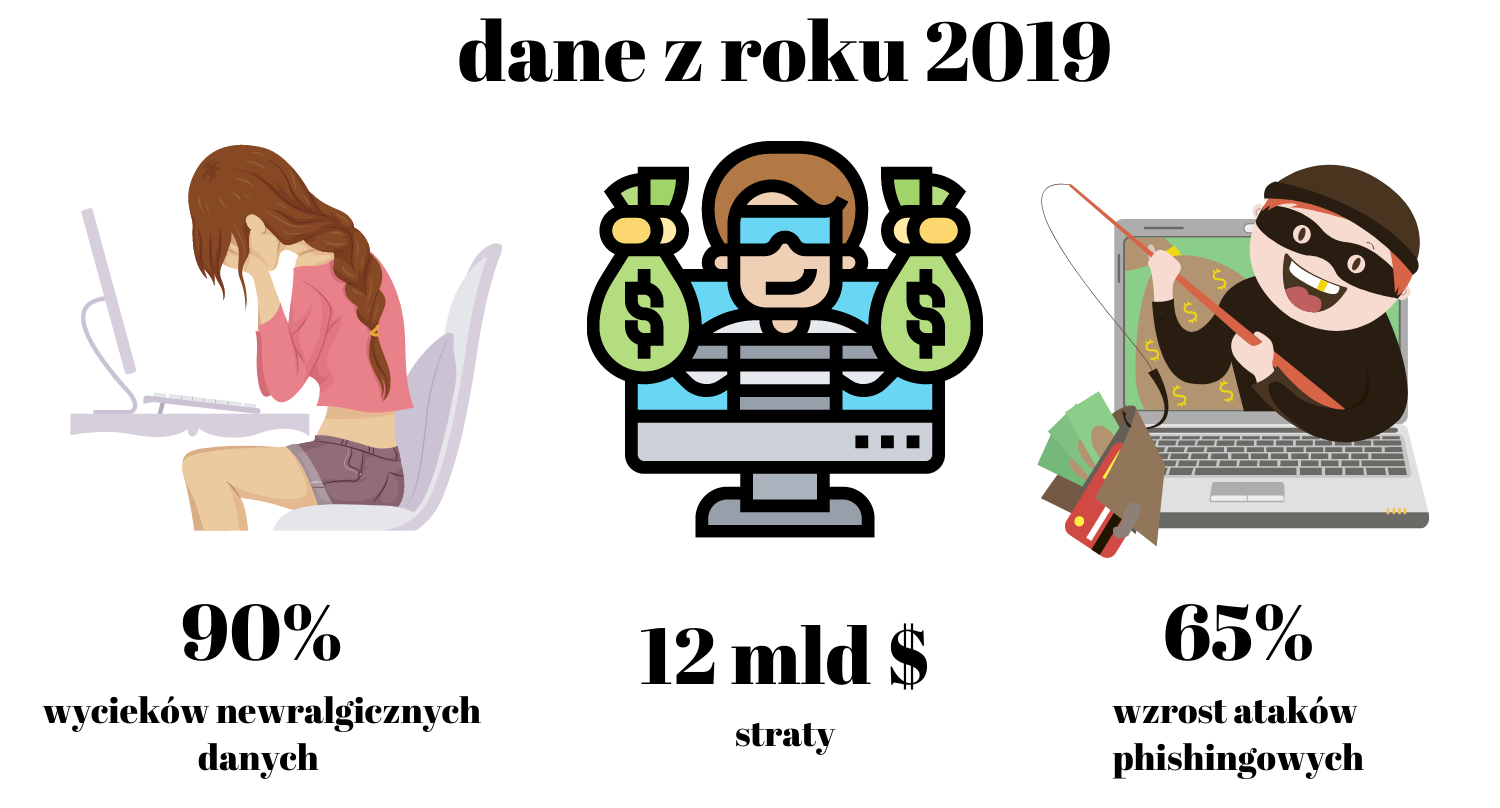
\includegraphics[width=1\linewidth]{../images/rys_2}
		\label{fig:rys2}
	\end{figure}
	Dane pochodzą z strony o \href{https://phishing.opcja.pl/}{kontrolowanym ataku phishingowym}.
\end{frame}

\section{Badane statystyki}
\begin{frame}
		
\end{frame}
\begin{frame}
	
\end{frame}

\section{Prezentacja kodu}
\begin{frame}
	\begin{center}
		\huge{Prezentacja kodu.}
	\end{center}
	\begin{figure}
		\centering
		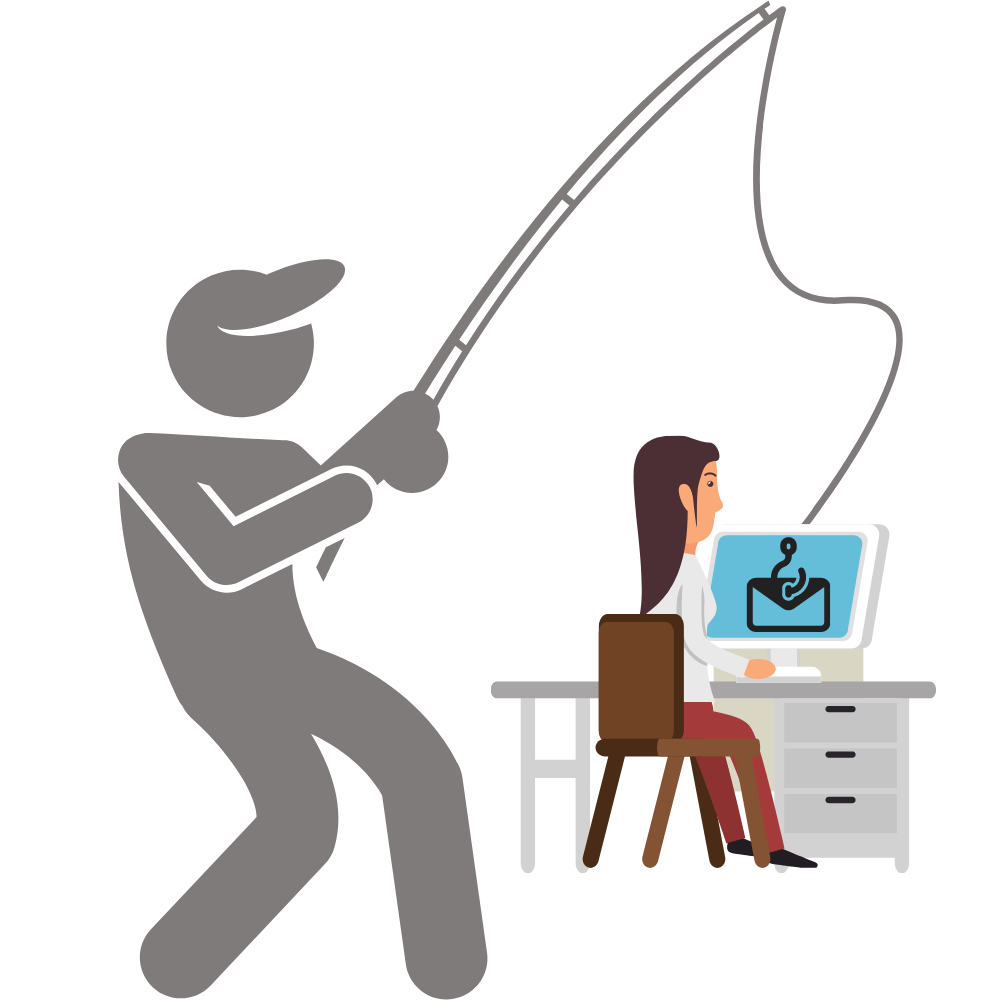
\includegraphics[width=0.5\linewidth]{../images/rys_6}
		\label{fig:rys6}
	\end{figure}
\end{frame}







\section{References}
\begin{frame}[allowframebreaks]{Literatura}
\begin{thebibliography}{}
	\setbeamertemplate{bibliography item}[online]
	\bibitem{1} 
	Kristiana Wijaya, Edy Tri Baskoro, Hilda Assiyatun, Djoko Suprijanto, \textit{Subdivision of graphs in $\mathcal{R}(mK_2,P_4)$}
\end{thebibliography}
\end{frame}

\end{document}